\section{Preliminaries}
\label{sec:preliminaries}
%
\subsection{Background}
\label{sec:background}
%
A data graph $G = (V,E,L)$ has a set of nodes $V$, a set of edges
$E \subseteq V \times V$, and a label set $\mathbb{L}$ s.t.
every node $v \in V$ is associated with a label, i.e., $L(v) \in \mathbb{L}$.
For simplicity, we focus on bidirectional, node labeled, and unweighted
graphs. However, the proposed models and algorithms can also be applied to weighted
and edge labeled graphs, e.g., in our experiments (\S~\ref{sec:experiments}), we demonstrate results over
edge labeled graphs.

\spara{Subgraph Isomorphism.} Given a data graph $G=(V,E,L)$, a graph pattern
$Q=(V_Q,E_Q,L_Q)$, a subgraph isomorphism is an {\em injective function} $M: V_Q \rightarrow V$ s. t.
{\bf (1)} $\forall v\in V_Q, L_Q(v)= L(M(v))$, and {\bf (2)} $\forall(v_1,v_2) \in E_Q, (M(v_1),M(v_2))\in E$.
%
\begin{figure}[t!]
\centering
\vspace{-1\baselineskip}
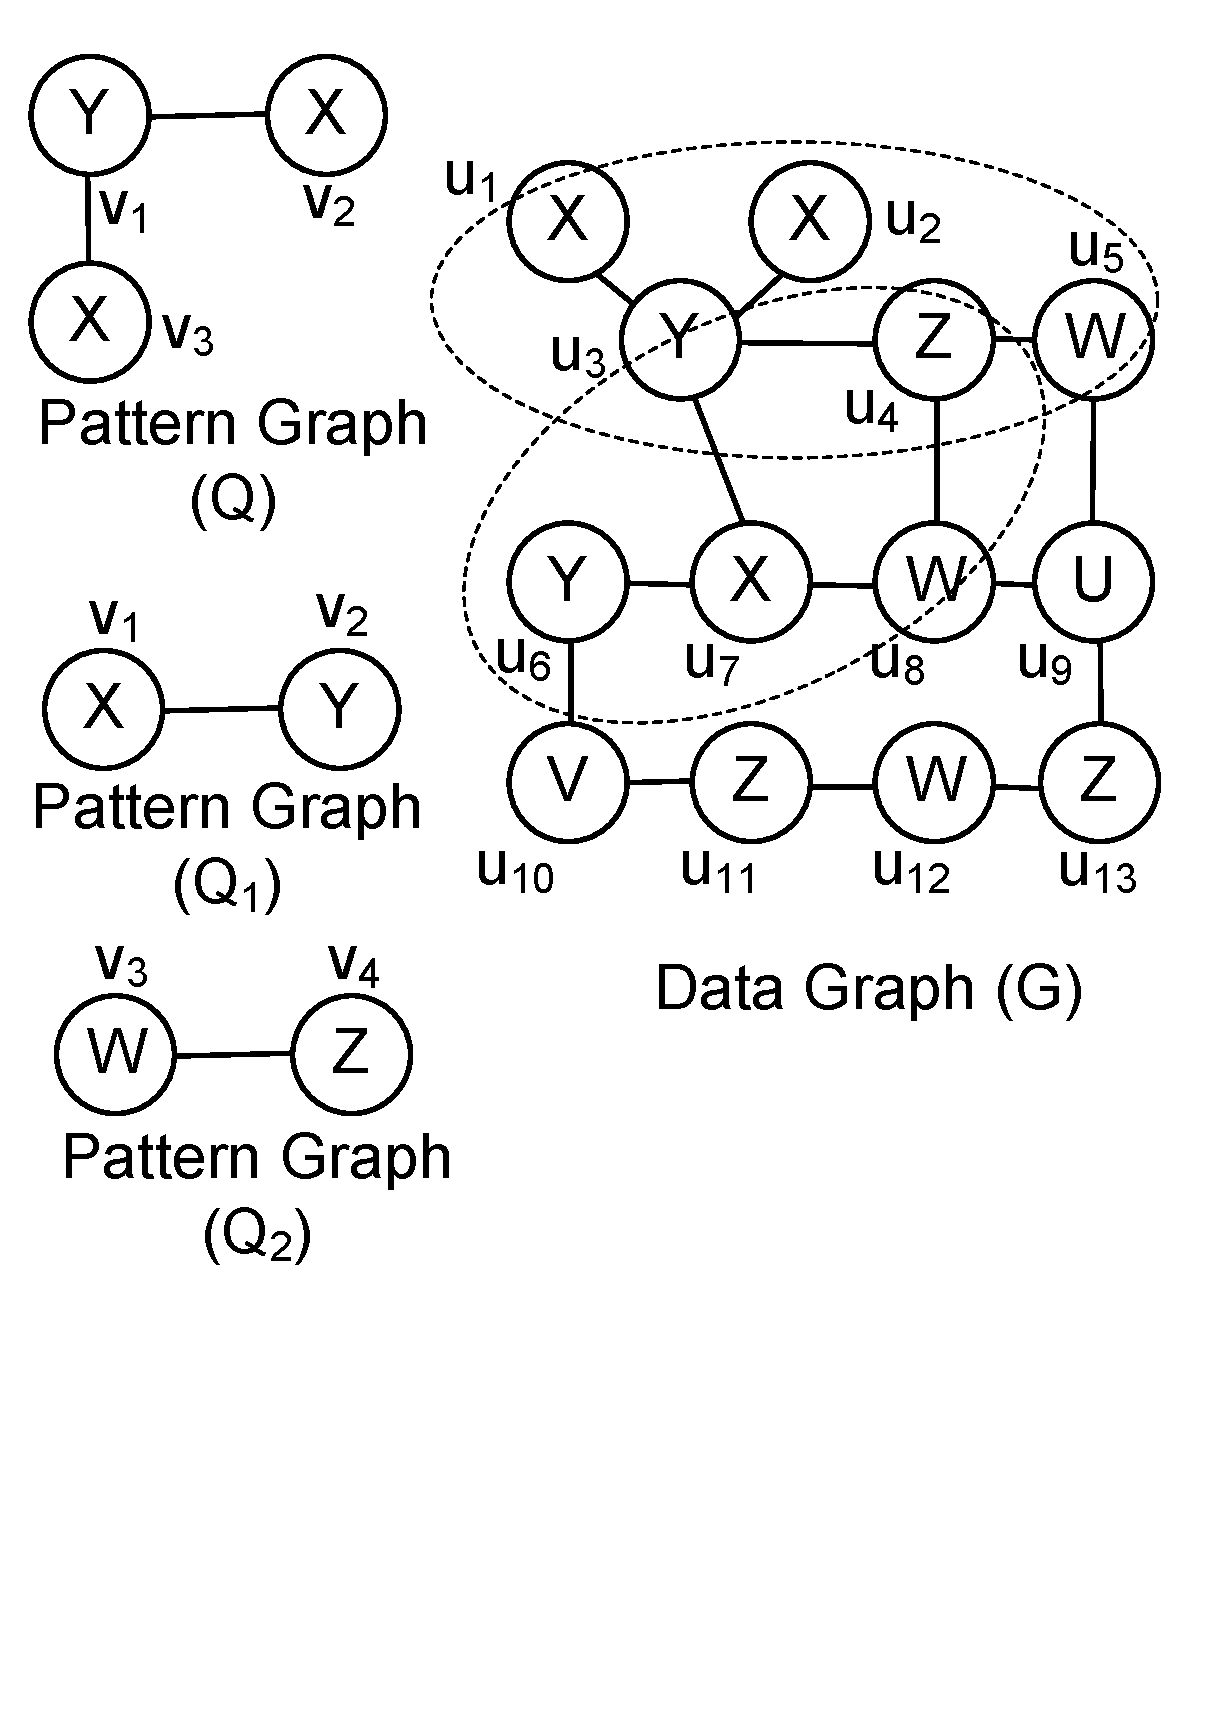
\includegraphics[scale=0.23]{images/correlation}
%\vspace{-1\baselineskip}
\caption{Subgraph isomorphism from $Q$ to $G$. Correlation between $Q_1$ and $Q_2$ in $G$.}
\label{fig:subgraph_isomorphism}
\vspace{-0.1\baselineskip}
\end{figure}

\spara{Support.}
To find frequent subgraphs\footnote{{\footnotesize We use `subgraph' and `subgraph pattern' interchangeably in the paper.}}
from a single, large graph, several definitions of subgraph support ($\sigma$)
have been proposed, e.g., maximum independent sets (MIS) \cite{KK04},
minimum image-based (MNI) \cite{BN08}, and harmful overlap (HO) \cite{FB07}.
We adopt MNI  \cite{BN08}
due to following reasons. {\bf (1)} MNI
can be efficiently computed from subgraph isomorphic instances;
whereas the computation of MIS and HO are \NP-complete \cite{KK04,FB07}.
{\bf (2)} MNI provides a superset of results of the two other metrics; thus
MIS or HO-based results can be identified via an expensive postprocessing step
\cite{EASK14}. {\bf (3)} MNI (as well as two other metrics) is {\em downward closure}:
The support of a supergraph $Q_1 \succeq Q$ is smaller (or equal) than that
of its subgraph $Q$, i.e., $\sigma(Q_1) \le \sigma(Q)$.

\spara{Minimum Image-based (MNI) Support \cite{BN08}.}
It is based on the number of unique nodes in $G$ that a node of the pattern $Q$
is mapped to. Formally,
%
\begin{align}
\displaystyle \sigma(Q) = \min_{v \in V_Q} |\{M(v) : M \,\text{is a subgraph isomorphic mapping}\}| \nonumber &
\end{align}
%
\begin{exple}
Figure~\ref{fig:subgraph_isomorphism} shows subgraph isomorphism. For a subgraph isomorphic
{\em mapping} $M$, the nodes $\{M(v):v\in V_Q\}$ and the corresponding edges $\{(M(v_1),M(v_2)):(v_1,v_2)\in E_Q\}$
form a subgraph isomorphic {\em instance} of $Q$ in $G$.
There can be many subgraph isomorphic mappings and instances, e.g.,
{\bf (1)} $M_1(v_1)= u_3$, $M_1(v_2)= u_2$, $M_1(v_3)= u_7$; {\bf (2)} $M_2(v_1) = u_3$, $M_2(v_2) = u_1$,
$M_2(v_3) = u_2$, etc. The MNI support of $Q$ is $1$, which is due to
node $v_1$: It is mapped to only one node in $G$, i.e., $u_3$ for all
mappings. The nodes in the set $\{M(v)\}$ for different mappings $M$ are called the {\em images} of $v$.
\end{exple}

\spara{Frequent Subgraphs.} Given the data graph $G$, a user-defined minimum support threshold $\Sigma$, and
a definition of support $\sigma$, the frequent subgraphs mining problem identifies all subgraphs $Q$ of $G$, such that
$\sigma(Q)\ge$ $\Sigma$.
%
\subsection{Problem Formulation}
\label{sec:problem}
%
Informally speaking, our objective is to identify those pairs of subgraph patterns $\langle Q_1, Q_2\rangle$ such that
they occur closely for a sufficiently large number of times in the data graph $G$. We formalize this notion of
correlation by incorporating the following constraints: {\bf (1)} The correlation between two subgraph patterns must be
symmetric, and {\bf (2)} it shall be consistent with the definition of MNI support.

For consistency with MNI, we group subgraph instances.
%
\begin{defn}[Instance Grouping]
\label{def:instance_grouping}
Given the data graph $G$, a graph pattern $Q$, and its instances in $G$ denoted as $\mathbb{I}=\{I_1,I_2,\ldots,I_s\}$,
let us define by $v^*$ the node in $Q$ which has the minimum number of images. We denote by
$\mathbb{M}(v^*)=\{M_1(v^*),M_2(v^*),\ldots,M_{\sigma(Q)}(v^*)\}$ the images of $v^*$. Notice that
$\sigma(Q)$ is the MNI support of $Q$, $\sigma(Q)\le s$, and $M_j(v^*)\in G$ is
a mapping of $v^*\in Q$, for all $1 \le j \le \sigma(Q)$. Next, we form a grouping
of instances, denoted as $\mathbb{I'}=\{I'_1,I'_2,\ldots,I'_{\sigma(Q)}\}$, where
$I'_j= \{I:M_j(v^*) \in I, I \in \mathbb{I}\}$. Intuitively,
$I'_j$ is the group of instances containing the image node $M_j(v^*)$.
\end{defn}
%
\begin{exple}
For data graph $G$ and graph pattern $Q_1$ in Figure~\ref{fig:subgraph_isomorphism},
the instances are
given by $\mathbb{I}=\{u_1u_3,u_2u_3,u_7u_3,u_7u_6\}$. However, its MNI support is two, since
node $v_2$ has only two corresponding images: $u_3$ and $u_6$. Thus, we group the instances
according to the presence of $u_3$ and $u_6$ as follows: $\mathbb{I'}=\{u_1u_2u_7u_3,u_7u_6\}$.
\end{exple}
%
%\begin{figure}[t!]
%\centering
%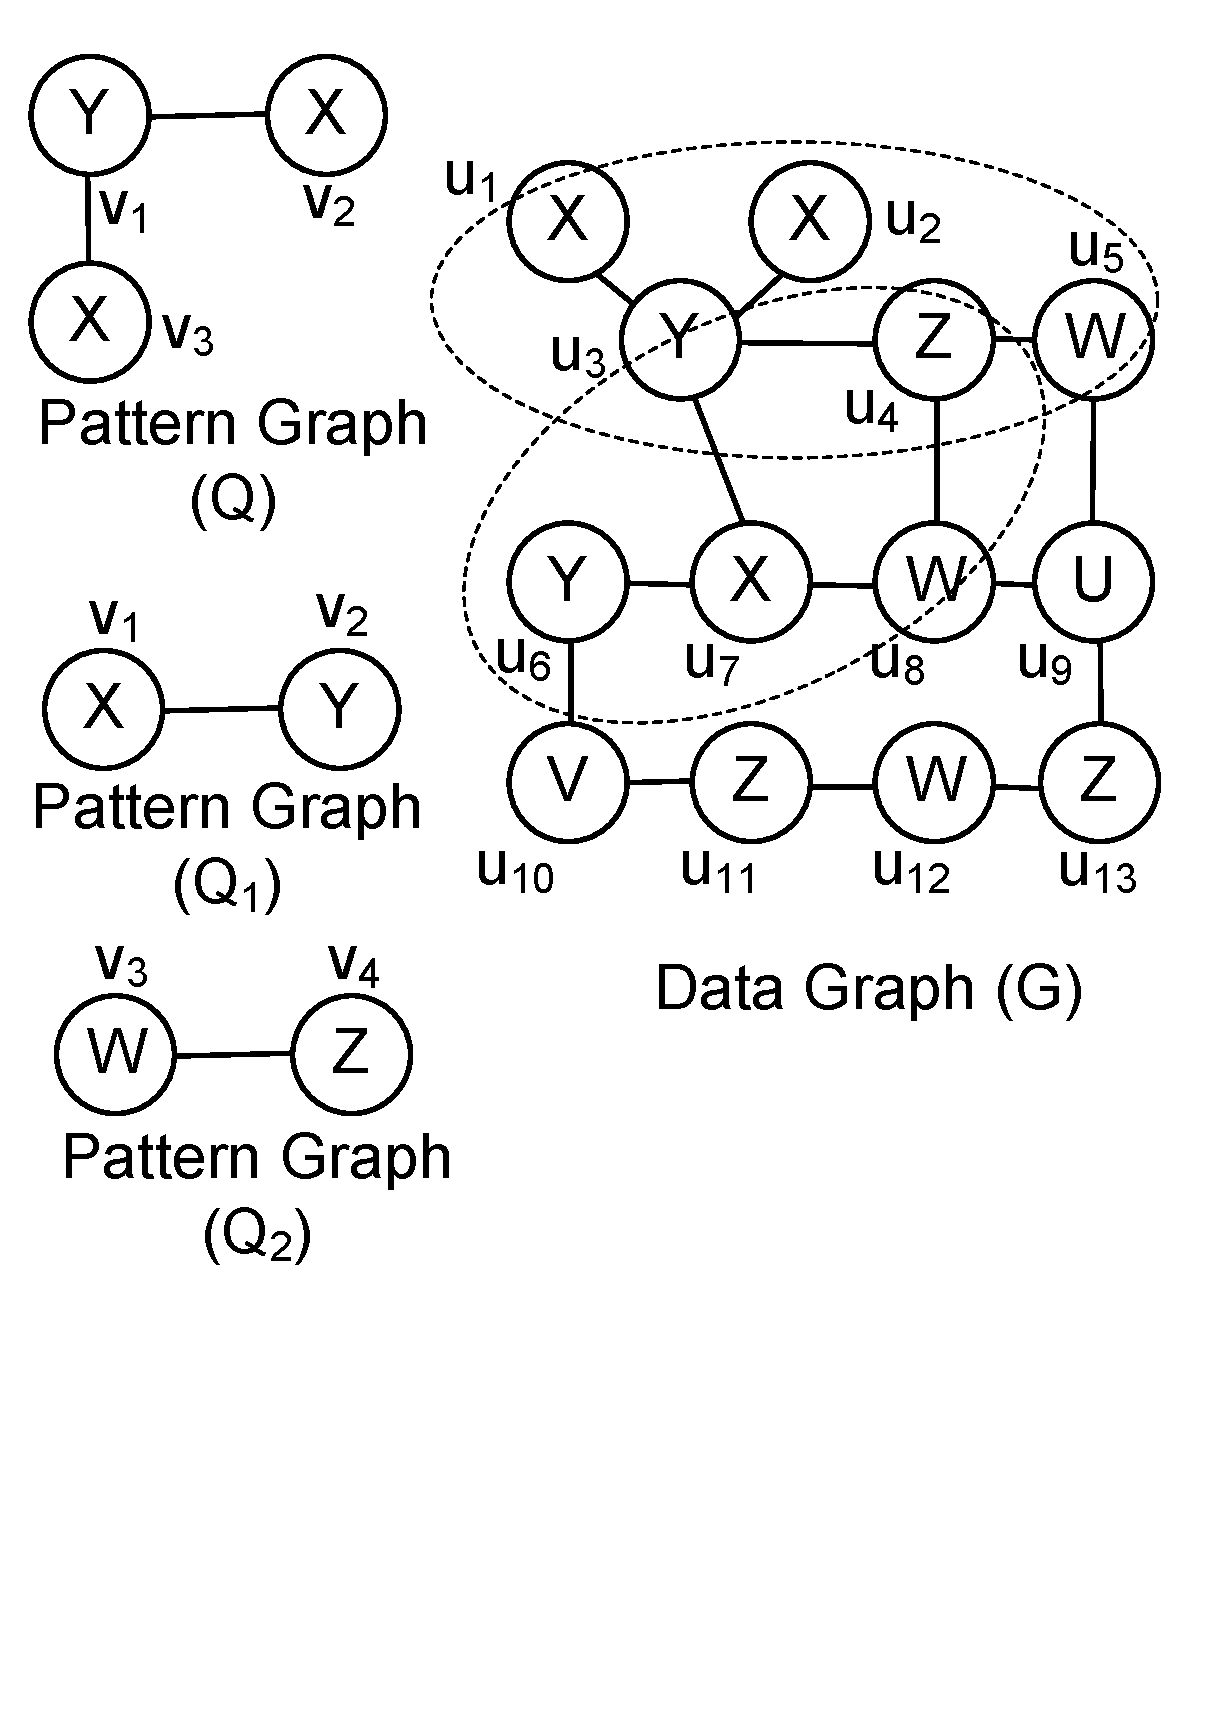
\includegraphics[scale=0.23]{images/correlation}
%\vspace{-1.75\baselineskip}
%\caption{Correlation between patterns $Q_1$ and $Q_2$ in $G$}
%\label{fig:correlation}
%\vspace{0.15\baselineskip}
%\end{figure}

Note that the grouping is not a partition of instances. It is possible for an instance
to belong to multiple groups, especially when the pattern has multiple nodes with the same label.
However, for a pattern $Q$, we ensure that the number of instance-groups would be $\sigma(Q)$.

Given two subgraph patterns $Q_1$ and $Q_2$, we compute their instance-groups:
$\mathbb{I'}=\{I'_1,I'_2,\ldots,I'_{\sigma(Q_1)}\}$ and $\mathbb{J'}=\{J'_1,J'_2,\ldots,$ $J'_{\sigma(Q_2)}\}$,
respectively. Without loss of generality, let us assume that $\sigma(Q_1) \le \sigma(Q_2)$.
Next, we count, out of all $\sigma(Q_1)$  instance-groups of $Q_1$, how many of them are ``close'' to at least
one instance-group of $Q_2$. We report this count as the {\em correlation} between $Q_1$ and $Q_2$ in $G$.
Finally, we define that two instance-groups $I' \in \mathbb{I'}$ and $J' \in \mathbb{J'}$
are close if there exist at least two nodes $u$ in $I'$ and $v$ in $J'$, such that their distance $d(u,v)\le h$,
that is, $u$ and $v$ are no more than $h$-hops away in the data graph $G$.
Clearly, $h\ge 0$ is a user-defined {\em distance threshold} parameter that can be varied to support different
amount of closeness between two co-occurrences of $Q_1$ and $Q_2$.
%
\begin{defn}[Correlation]
\label{def:correlation}
Given two patterns $Q_1$ and $Q_2$ in the data graph $G$, their instance-groups
$\mathbb{I'}=\{I'_1,I'_2,\ldots,$ $I'_{\sigma(Q_1)}\}$ and $\mathbb{J'}=\{J'_1,J'_2,\ldots,$ $J'_{\sigma(Q_2)}\}$,
respectively, and a user-defined distance threshold $h\ge0$,
assume that $\sigma(Q_1) \le \sigma(Q_2)$. We define the correlation
$\kappa(Q_1,Q_2,h)$ as:
%
\begin{align}
&\kappa(Q_1,Q_2,h) \nonumber & \\
&= |\{I' \in \mathbb{I'}:\exists J' \in \mathbb{J'}, \exists u \in I', \exists v \in J', d(u,v)\le h\}| \nonumber &
\end{align}
\end{defn}

The correlation, for the case $\sigma(Q_2) < \sigma(Q_1)$, can be defined analogously.
We note that the correlation between two subgraphs $Q_1$ and $Q_2$ is {\em symmetric}, that is,
$\kappa(Q_1,Q_2,h)$ = $\kappa(Q_2,Q_1,h)$.
%
\begin{exple}
Let us consider two subgraph patterns $Q_1$ and $Q_2$ in the data graph $G$ (Figure~\ref{fig:subgraph_isomorphism}),
and the distance threshold $h=1$. The instance-groups of $Q_1$ are given by: $\mathbb{I'}=\{u_1u_2u_7u_3,u_7u_6\}$,
where the groupings are performed based on the images of node $v_2$ in $Q_1$. Similarly,
the instance-groups of $Q_2$ are given by: $\mathbb{J'}=\{u_5u_4, u_8u_4,u_{11}u_{12}u_{13}\}$,
here the groupings are performed based on the images of node $v_3$ in $Q_2$. We have,
$\sigma(Q_1) =2 < \sigma(Q_2) =3$. Thus, we count, out
of two instance-groups of $Q_1$, how many of them are within $h=1$-hop of at least
one instance-group of $Q_2$. This gives us the correlation $\kappa(Q_1,Q_2,h=1)=2$.
\end{exple}

We are now ready to define our problem formally.
%
\begin{problem}
\label{prob:top-k}
{\bf {\sf Top-$k$} Correlated Subgraphs Mining (}{\sf{CSM}}{\bf).}
Given the data graph $G$, a user-defined distance threshold $h\ge0$, a minimum support threshold $\Sigma$, find the {\em top-$k$} pairs of subgraph patterns $\langle Q_1, Q_2 \rangle$ of $G$, having the
maximum correlations $\kappa(Q_1,Q_2,h)$, and for each subgraph pattern $\sigma(Q_1)\ge \Sigma$, $\sigma(Q_2)\ge \Sigma$.
\end{problem}

Analogous to the {\em association rule mining} over a transaction dataset \cite{AS94}, we consider both: {\bf (1)} a {\em minimum
support threshold} $\Sigma$ such that each constituent subgraph pattern is individually frequent, and {\bf (2)} a {\em correlation
measure} between a pair of frequent subgraph patterns so to identify the top-$k$ pairs based on their
correlations. Notice that {\bf (i)} if $Q_1$ is a subgraph of $Q_2$, or vice versa, the correlation between them is not interesting.
Thus in our methods, we remove those pairs which are related by subgraph and supergraph relationships.
Similarly, {{\bf (ii)} if $Q_1$ and $Q_2$ have high correlation {\em only} because they are subgraphs of a frequent
pattern $Q_3$, i.e., $Q_3 \succeq Q_1$ and $Q_3 \succeq Q_2$, such correlations are also not interesting. In our solution
framework, we devise a technique to detect and eliminate such subgraph pairs from our top-$k$ result.
%
%
\subsection{Theoretical Characterization}
\label{sec:characteristics}
%
The correlation metric satisfies several interesting properties.
%
\begin{lma}
\label{lemma:downward}
Correlation metric $\kappa(Q_1,Q_2,h)$ is not downward closure. Specifically, consider that $Q_3$ is a subgraph of $Q_2$, i.e.,
$Q_2 \succeq Q_3$. Then the following $\kappa(Q_1,Q_3,h) \ge \kappa(Q_1,Q_2,h)$ does not always hold.
\end{lma}
%
The downward closure property does not always hold because as one grows the size of the pattern (e.g., from $Q_3$ to $Q_2$), the super pattern
$Q_2$ may now have larger size instances that are closer to the instances of the other pattern $Q_1$.
In Figure~\ref{fig:subgraph_isomorphism}, let us consider
$Q_3$ as a single node with label $W$, whereas the patterns $Q_1$ and $Q_2$ are shown in the figure. Clearly, $Q_2 \succeq Q_3$.
We notice that $\kappa(Q_1,Q_3,h=1)=1$ and $\kappa(Q_1,Q_2,h=1)=2$. Hence, the downward closure property does not always hold.
%
\begin{lma}
\label{lemma:upward}
Correlation metric $\kappa(Q_1,Q_2,h)$ is not upward closure. In particular, consider that $Q_4$ is a supergraph of $Q_1$, i.e.,
$Q_4 \succeq Q_1$. Then the following $\kappa(Q_1,Q_2,h) \le \kappa(Q_4,Q_2,h)$ does not always hold.
\end{lma}
%
The upward closure property does not always hold because as one grows the size of the pattern (e.g., from $Q_1$ to $Q_4$), the super pattern
$Q_4$ may naturally have lower MNI support (and, hence smaller number of instance-groups).
This can reduce its correlation with the other pattern $Q_1$.
In Figure~\ref{fig:subgraph_isomorphism}, let us consider $Q_4$ consisting of three nodes $X-Y-X$,
whereas the patterns $Q_1$ and $Q_2$ are shown in the figure. Clearly, $Q_4 \succeq Q_1$.
We notice that $\kappa(Q_1,Q_2,h=1)=2$ and $\kappa(Q_4,Q_2,h=1)=1$. Hence, the upward closure property does not always hold.

Since upward and downward closure properties are widely used in frequent pattern mining problems \cite{AS94,KK01,BN08,FB07,KK04,YH02}
--- in particular, for early termination of the proposed algorithms, Lemma~\ref{lemma:downward} and \ref{lemma:upward} demonstrate the inherent
complexity of our {\sf{CSM}} problem.

Fortunately, Lemma~\ref{lemma:prune} would be useful to design an early termination criteria in our algorithm.
%
\begin{lma}
\label{lemma:prune}
The following inequality holds: $\kappa(Q_1,Q_2,h) \le \min \{\sigma(Q_1),\sigma(Q_2)\}$.
\end{lma}

Lemma~\ref{lemma:prune} directly follows from the definition of correlation (Definition~\ref{def:correlation}), which is computed
from the instance-groups of that subgraph pattern having the smaller support. 